\chapter{Background, Definitions and Notations}
\epigraph{
  I can't go to a~restaurant and order food because I keep looking at the fonts on~the menu.
}{Donald Ervin Knuth}

\section{General Game Theory}

\subsection{What Is Game Theory?}

The field of Game Theory deals with interactions or conflicts between $2$ or more agents.
\todo

A~\emph{(simultaneous move) game} consists of: \todo
\begin{itemize}
  \item set $P$ of players $\braces{1, 2, \cdots, n}$
  \item actions
  \item payoffs
\end{itemize}

There are additional concepts related to games such as: \todo
\begin{itemize}
  \item \emph{strategy}
  \item \emph{dominant strategy}
  \item \emph{best response}
  \item \emph{pure Nash equilibrium}
  \item \emph{mixed strategy}
  \item \emph{(mixed) Nash equilibrium}
  \item \emph{correlated equilibrium}
\end{itemize}

A~\emph{game with turns} has:
\begin{itemize}
  \item \todo
\end{itemize}

\subsection{Representation of Games}

\todo
\begin{itemize}
  \item standard (matrix) form
  \item compactly represented game
\end{itemize}

There will be other kinds of representation for extensive form games (see Subsection~\ref{ssec:extensive-form}).

\subsection{Standard Examples}

\todo %Describe the games and how the game-theoretic definitions from above look like in these examples

\begin{itemize}
  \item{Rock-paper-scissors}
  \item{Chess}
  \item{Poker}
\end{itemize}

\section{Combinatorial Game Theory}
\label{sec:CGT}

\todo

\section{The Game of Go}
\label{sec:Go}

\subsection{Rules}

\emph{Black} and \emph{White} place pieces (\emph{stones}) on the unoccupied intersections (\emph{points}) of a~\emph{board} with a~$19\times19$ grid of~lines.
Players take turns, Black moves first.
There are only 2 basic rules of Go:
\begin{description}
  \item [The rule of liberty]
    Every stone remaining on the board must have at least one open point (an~intersection, called a~\emph{liberty}) directly next to it (up, down, left, or right), or must be part of a~connected group that has at least one such liberty next to it.
    \begin{figure}[H]
      \centering
      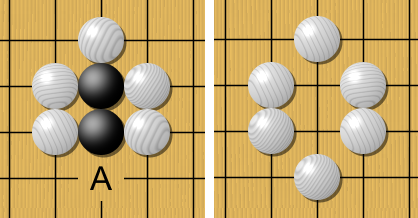
\includegraphics[width=.5\textwidth]{../img/Go_rule_of_liberty.png}
      \caption{The rule of liberty}
      \label{fig:Go-rule-liberty}
    \end{figure}

    Stones or groups of stones which lose their last liberty are removed from the board.

  \item [The ``ko'' rule]
    The stones on the board must never repeat a~previous position of~stones.
    This is to prevent unending cycles.
    \begin{figure}[H]
      \centering
      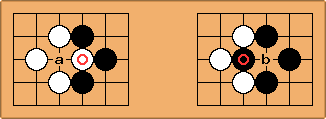
\includegraphics[width=.5\textwidth]{../img/Go_ko_rule.png}
      \caption{The ``ko'' rule}
      \label{fig:Go-Ko-rule}
    \end{figure}

\end{description}

\subsection{Scoring, Ranks and Handicaps}

There are several \textbf{scoring rules} to determine the winner of a~game.
In the match of~AlphaGo against Lee Sedol,%
\footnote{See Chapter~\ref{ch:AlphaGo}.}
the \emph{area scoring} was used.
Under area scoring system, player's score is:
\begin{itemize}
  \item the number of stones that the player has on the board
  \item plus the number of~empty intersections surrounded by that player's stones
  \item plus \emph{komi(dashi)} points%
    \footnote{a~compensation for the first move advantage of~the Black player}
    for the White player
\end{itemize}

\emph{Elo rating} can be used to denote players' \textbf{ranks}.
Alternatively, \emph{kyu/dan} (in~Japanese) or \emph{gup/dan} (in~Korean) system is also vastly popular:
\begin{figure}[H]
  \centering
  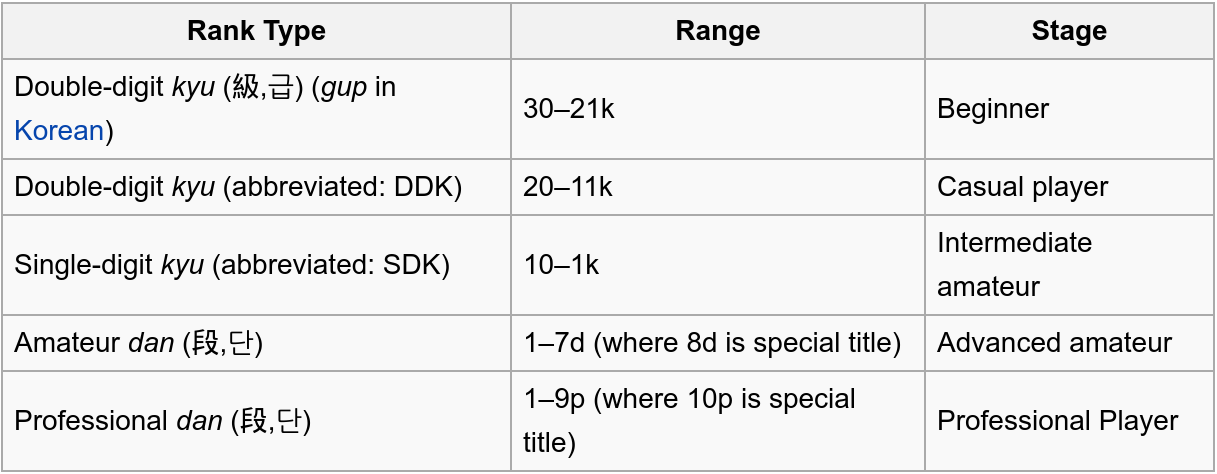
\includegraphics[width=.8\textwidth]{../img/Go_kyu_dan.png}
  \caption{Kyu/Gup and Dan ranks}
  \label{fig:Go-ranks}
\end{figure}

\textbf{Handicap} system is used to even up differences in ranks:
Black can place 1 or more stones in advance as a~compensation for White's greater strength.

\section{Algorithmic Game Theory}

\subsection{What Is Algorithmic Game Theory?}
One of the classic textbook is the extensive \emph{Algorithmic Game Theory} (\cite{AGT07}).
\todo

\subsection{Examples from Algorithmic Game Theory}

The following games capture various game-theoretic properties and the ``real-life'' counterparts of these games in the fields such as networking, economy etc.
The examples and figures are taken from \emph{Algorithmic Game Theory} (\cite{AGT07}).

\newcommand{\widthratio}{0.3}
\begin{itemize}
  \item \emph{Prisoner's dilemma} \todo
    \begin{figure}[H]
      \centering
      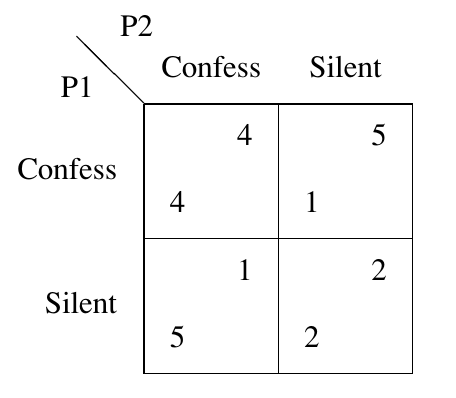
\includegraphics[width=\widthratio\paperwidth]{../img/prisoner.png}
      \caption{Prisoner's dilemma}
      \label{fig:prisoner}
    \end{figure}

    \begin{figure}[H]
      \centering
      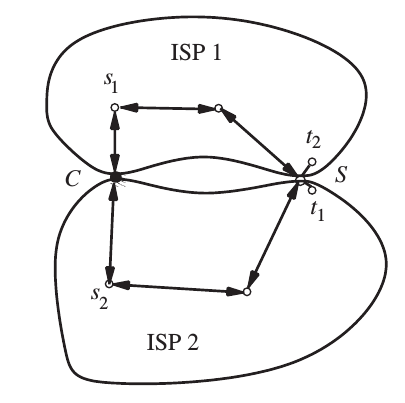
\includegraphics[width=\widthratio\paperwidth]{../img/isp.png}
      \caption{ISP routing game}
      \label{fig:isp-routing}
    \end{figure}


  \item \emph{Pollution game} is a multi-player version of Prisoner's dilemma \todo

  \item An~example of a~coordination game is the \emph{Battle of sexes}.

    \begin{figure}[H]
      \centering
      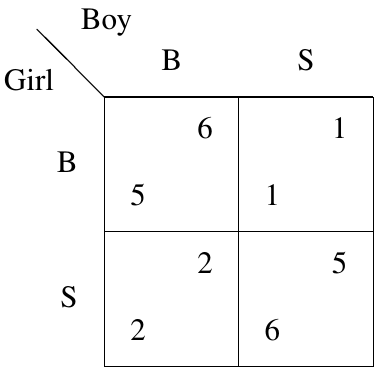
\includegraphics[width=\widthratio\paperwidth]{../img/battle-of-sexes.png}
      \caption{Battle of sexes}
      \label{fig:battle-of-sexes}
    \end{figure}

  \item Another coordination game is the \emph{Routing congestion game}, taken from the world of networking

    \begin{figure}[H]
      \centering
      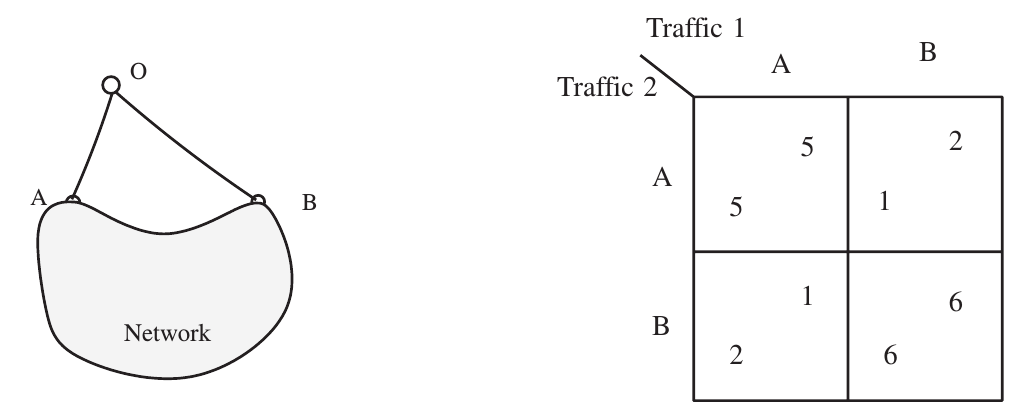
\includegraphics[width=0.65\paperwidth]{../img/routing-congestion-game.png}
      \caption{Routing congestion game}
      \label{fig:routing-congestion}
    \end{figure}

  \item \emph{Matching pennies} can be considered as a $2$-choice reduction of Rock-paper-scissors.

    \begin{figure}[H]
      \centering
      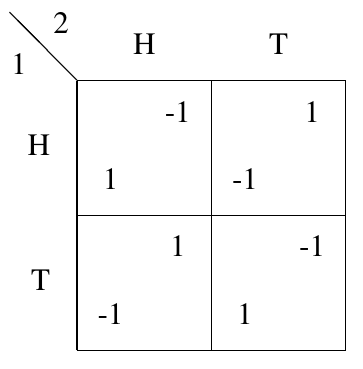
\includegraphics[width=\widthratio\paperwidth]{../img/matching-pennies.png}
      \caption{Matching pennies}
      \label{fig:matching-pennies}
    \end{figure}

  \item \emph{Pricing game} is an~example of a~game without a~(mixed) Nash equilibrium.

    \begin{figure}[H]
      \centering
      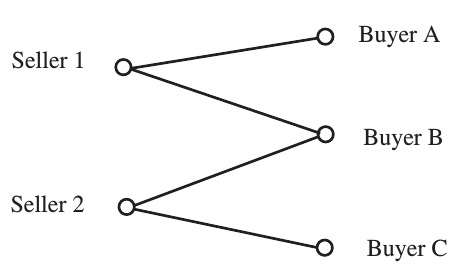
\includegraphics[width=\widthratio\paperwidth]{../img/pricing-game.png}
      \caption{Pricing game}
      \label{fig:pricing-game}
    \end{figure}

  \item \emph{Traffic light}

    \begin{figure}[H]
      \centering
      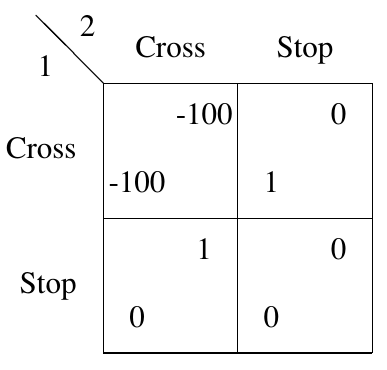
\includegraphics[width=\widthratio\paperwidth]{../img/traffic-light.png}
      \caption{Traffic light}
      \label{fig:traffic-light}
    \end{figure}

  \item \emph{Ultimatum game}
\end{itemize}

\subsection{Extensive Form}
\label{ssec:extensive-form}

An \emph{extensive-form game} consists of

\begin{itemize}
  \item a finite set of \emph{players} $P$,
  \item a finite set $H$ of all possible \emph{histories},
    \begin{itemize}
      \item Each history consists of individual \emph{actions}.
      \item $h \sqsubseteq h'$ denotes that history~$h$ is a~prefix of $h'$.
      \item $\emptyset \in H$ and $h' \in H \land h \sqsubseteq h' \implies h \in H$
      \item Set $Z \subseteq H$ is the set of \emph{terminal histories}, i.e. histories that are not prefixes of any other histories.
    \end{itemize}
  \item the set of available actions $A(h) = \braces{a: (h, a) \in H}$ for every node $h \in H \setminus Z$,
  \item a~function $P()$ assigning an~\emph{acting player} to each $h \in H \setminus Z$.
    The acting players are taken from the set $P \cup \braces{c}$, where $c$ is the \textbf{c}hance player (e.~g. a~dice, the card dealer, the nature etc.).
    Thus, $P(h) \in P \cup \braces{c}$ for any $h \in H \setminus Z$.
  \item a~function $f_c$ determining the probability measure over actions $A(h)$ for nodes $h$ with $p(h) = c$, the nodes of the chance player.
  \item The partition $\I_i$ of nodes $\braces{h \in H: p(h) = i}$ is called the \emph{information partition} of player~$i$.
    Its element $I \in \I_i$ is an \emph{information set} of player~$i$ and $I(h) \in \I_i$ (with $p(h) = i$) denotes the information set containing $h$.

    An information set represents grouping of histories that are indistinguishable from $i$'s point of view.
    In the game of poker, for example, this might be because of hidden cards of opponents.
  \item a \emph{utility function} $u_i\colon Z \goto \R$,
\end{itemize}

There are further notions related to any extensive-form game:

\begin{itemize}
  \item \emph{Strategy}~$\sigma_i$ of (non-chance) player~$i$ determines a~probability distribution over $A(I)$ at every $I \in \I_i$.
    Thus $\pi ^\sigma (I, a)$ is the probability of action $a$ at the information set~$I$.
    $\Sigma_i$ denotes the set of all possible strategies for player~$i$.
  \item A~\emph{strategy profile} is a~vector of all (non-chance) players' strategies denoted by $\sigma = (\sigma_1, \sigma_2, \ldots, \sigma_ {\abs{P}})$.
    The set of all such possible strategy profiles is denoted by $\Sigma$.
    Hence, it is the Cartesian product $\Sigma = \prod\limits _{i \in P} \Sigma_i$.
  \item We use the Greek letter $\pi$ to evaluate the probability corresponding to a~profile~$\sigma$:
    \[\pi ^\sigma(h) = \prod _{i \in P \cup \braces{c}} \pi _i ^\sigma (h)\]
    
  \item The probability $\pi _{-i} ^\sigma (h)$ (or sometimes just briefly $\pi _{-i} (h)$) is the product of~all players' contribution, except for the one of player~$i$:
    \[\pi _{-i} ^\sigma(h) = \prod _{j \in P \setminus \braces{i} \cup \braces{c}} \pi _j ^\sigma (h)\]
    
  \item $\sigma | _{I \goto a}$ denotes the strategy identical to $\sigma$ with the only one exception:
    the action~$a$ is always played at the information set~$I$.
  \item Given the strategic profile $\sigma$, the \emph{expected utility}~$u_i (\sigma)$ for player~$i$ is defined as:
    \[ u_i (\sigma) = \sum _{z \in Z} \pi ^\sigma (z) u_i(z)\]

  \item A~\emph{best response} $BR _i (\sigma _{-i})$ (or briefly $BR _i (\sigma)$) of player $i$ for given $\sigma _{-p}$ is such a~strategy $\sigma _i \in \Sigma _i$ that maximizes player's expected utility against others:
    \[ u_i (\sigma) = \max _{\sigma'_i \in \Sigma_i} u_i ((\sigma'_i, \sigma_{-i})) \]

  \item A~\emph{Nash equilibrium} (in the context of extensive-form games) is a~strategy profile $\sigma$ such that no player~$i \in P$ has any incentive to deviate from his strategy.
    In other words, all players are playing best responses against each other:
    \[ \forall i \in P\colon u_i (\sigma) = \max _{\sigma'_i \in \Sigma_i} u_i ((\sigma'_i, \sigma_{-i})) \]

  \item The \emph{counterfactual value} $v _i ^\sigma (I)$ is the expected utility provided that the information set $I$ is reached and all players play according to strategy $\sigma$ with exception of player~$i$, who plays to reach $I$:
    \[ v _i ^\sigma (I) = \sum\limits _{h \in I, \; h' \in Z}
      \frac
      {\pi _{-i} ^\sigma(h) \pi ^\sigma(h,h') u_i(h')}
      {\pi _{-i} ^\sigma (I)} \]

  \item A~\emph{counterfactual best response} $CBR _i (\sigma _{-i})$ (or briefly $CBR _i (\sigma)$) of player~$i$ is a~strategy maximizing the counterfactual value at each information set $I \in \I _i$:
    \[ \pi ^\sigma (I, a) \geq 0
      \; \Longleftrightarrow \;
      v _i ^\sigma (I, a) = \max _{a' \in A(I)} v _i ^\sigma (I, a') \]

    Note that $CBR _i (\sigma)$ is always a best response $BR _i (\sigma)$, but the reverse implication does not need to hold:
    a~best response $\sigma$ can select an~arbitrary action in an~unreachable information set $I$ (the one where $\pi ^\sigma (I) = 0$).
    Such best responses are in general not counterfactual best responses.

  \item For the sake of notation's simplicity, we will define \emph{counterfactual best response value} as the counterfactual value for the strategy, where player $i$ plays according $CBR _i (\sigma _{-i})$ rather than the original $\sigma$.
    Formally, it is
    \[ CBV _i ^\sigma (I) = v _i ^{(\sigma _{-i}, CBR _i (\sigma _{-i} ))} (I) \]

\end{itemize}

There may be various properties for extensive-form games:

\begin{itemize}
  \item being \emph{two-player}
  \item having \emph{perfect recall}: any two states from the same information set $I \in \I _i$ share the same history of past actions and player $i$'s information sets.

    In other words, at any stage of the game no player can forget what happened so far:
    neither actions taken nor the information sets reached.
  \item being \emph{zero-sum}: For any $\sigma \in \Sigma$ we have $\sum _{i \in P} u _i (\sigma) = 0$.
\end{itemize}

\subsection{Sequence Form}

\section{Methods of~Solution}

\subsection{Linear Programming}
{
  \setlength{\epigraphwidth}{0.65\textwidth}
  \epigraph{
    If you optimize everything, you will always be unhappy.
  }{Donald Ervin Knuth}
}

\subsection{Learning}
\epigraph{
  Perfecting oneself is as~much unlearning as~it is learning.
}{Edsger Dijkstra}

\section{Subgames (Endgames)}

So far, the information sets have grouped only those states where the player was the acting player.
For the purposes of the subgame, it is also necessary to include the states that are indistinguishable from the point of view of other players.
Therefore, we define the \emph{augmented information sets} (\cite{BurchJohansonBowling13}):

\begin{itemize}
  \item For any player $i \in P$, let $H_i(h)$ be the sequence of player $i$'s information sets reached by player $i$ on the path to $h$, and the actions taken by player~$i$.
  \item An~\emph{augmented information set} $I_i(h)$ is defined by the following characterization:
    for any two states $h, h' \in H$, we have that 
    \[ I_i (h) = I_i (h') \; \Longleftrightarrow \; H_i (h) = H_i (h') \]
\end{itemize}

At this point, we may finally define the notion of a~\emph{subgame}:

\begin{itemize}
  \item An~(imperfect information) \emph{subgame} is a~forest of trees, closed under both the descendant relation and membership within augmented information sets for any player (\cite{BurchJohansonBowling13}).
\end{itemize}

\subsection{Previous Works}
